\documentclass[11pt,a4paper]{article}
% Doc settings
    \usepackage[margin=2.3cm]{geometry}
    \usepackage{xcolor}
    \usepackage{amsmath}
    \usepackage{csquotes}
    \usepackage{setspace}
    \usepackage{url}
    \usepackage{graphicx}
    \usepackage{geometry}
    \usepackage{subcaption}
    \usepackage{caption}


    \setstretch{1.4}    % Set line spacing to 1.5 times the font size
    \raggedbottom       % Remove extra vertical space between sections

\begin{document}

% Title Page
\begin{titlepage}
    \centering
    \vspace*{2cm}
    {\LARGE Information Shocks and the Global Financial Cycle \par}
    \vspace{2cm}
    {\large Jessica Cremonese \par}
    \vspace{1cm}
    {\large Università degli Studi di Padova \par}
    \vspace{1cm}
    {\large Applied Macroeconomics (Mod. B) - 2022-2023 \par}
    \vspace{1cm}
    {\large Date: \par}
    {\large \today \par}
\end{titlepage}


\newpage
\section{Introductory remarks}    
Unprecedented financial globalization, coupled with the emergence of global intermediaries, has profoundly influenced the functioning of national financial markets and the transmission mechanisms of policy shocks among increasingly interconnected nations.
The United States dollar has traditionally held a position of unrivaled dominance in the international arena, to such an extent that US monetary policy has been observed to have spillover effects on other economies.
Due to the extensive dollar-denominated assets, domestic decisions significantly impact the portfolios of major global banks, thereby affecting lending and credit choices, corporate spreads, price levels, and agents' risk propensity.
For this reason, macroeconomists are increasingly interested in understanding the movements of capital flows and the transmission of policy across borders. 

% WHAT IS A PRICE PUZZLE?
In the study of monetary policy (MP) shocks, a \enquote{price puzzle} refers to a situation where the response of prices to a MP shock is inconsistent with the predictions of standard economic theory. Specifically, it refers to an unexpected short-term relationship between MP actions and the behavior of prices and output. 
A contractionary MP shock, such as an increase in interest rates, is expected to dampen aggregate demand and result in lower output and inflation. However, researchers have found instances where the response of prices to MP shocks is contrary to these expectations. 
Understanding the causes and implications of price puzzles is crucial for improving our understanding of the dynamics of MP and its impact on the economy.

% MAREY 2020
A recent paper by Miranda-Agrippino and Rey (2020) the interplay of US monetary policy and the existence of a Global Financial Cycle (GFC). 
The authors analyse the transmission of MP shocks via a rich information Bayesian VAR with an external instrument, which claims to reduce issues of omitted variables and manage imperfect information. 
        % MA IN REALTA' NON RIESCONO PERCHE' SI ASSUME CHE CB HA PERFECT INFORMATION, MA NON E' COSI'
MP shocks are identified from high-frequency asset prices adjustments around FOMC (Federal Open Market Committee) announcements. 
Such an instrument is valid only under the assumption that market agents can correctly discern monetary policy decisions from policy actions. If informational asymmetries are present, the high-frequency surprises are also a funcion of the \enquote{FED information effect}: information shocks about the economic fundamentals that are implicitly conveyed by the central bank's announcements. 
Thus, the authors are using central bank's (CB) announcements to isolate the MP shocks. However, they assume that announcements are also informative with respect to the CB's internal macroeconomic assessment. 


% results of MAREY (2020)
The findings show the existence of a common global factor which accounts for roughly 20\% of the variability in prices of risky assets. 
In terms of domestic responses, they report that a contractionary shock depresses prices and output, and housing investments, accompanied by an increase in unemployment.
significantly, their work highlights a distinct reaction in global prices of risky assets, indicating the existence of spillover effects.
Specifically, following a contraction in US monetary policy, there is an upsurge in risk aversion, a substantial reduction in credit provision, and a decrease in global capital inflows. Global intermediaries react faster than domestically oriented retail banks, however contract leverage.


% MARICCO 2021    
In the presence of incorrect accounting for imperfect information, the estimated dynamic responses to shocks are dependent on the choice of instrument, sample and empirical specification of choice. Miranda-Agrippino and Ricco (2021) propose an identification strategy that is robust to the presence of imperfect information between the public and the CB.
High-frequency market based surprises around policy announcements tend to correlate with the CB's private macroeconomic forecasts. Consequently, they define the unexpected component of monetary policy shocks as the exogenous shifts in the policy instrument that surprise market participants and are unforecastable, as well as being uncorrelated with the CB's systematic response to the macroeconomic outlook.  This allows to disentangle monetary policy actions from information shocks. 
Their results show behavior of dynamic responses coherent with economic theory and no evidence of output or price puzzles. Furthermore, they find that a monetary contracion is unequivocally and significantly recessionary, with output contracting immediately and significantly, as well as prices, domestic demand, labor market conditions, investments and household wealth. There is evidence of a credit channel which magnifies these effects through credit provision and financial markets, the yield curve flattens, borrowing costs and corporate spreads rise.

% secondo Dario:
% limite di REY: external instrument IV + 
    %%          NON TIENE CONTO DEL SIGNALING EFFECT DELLA CB !!!
% RICCO usa proxy, quindi proxy entra come variabile

In order to estimate the effect of an information shock on the GFC and a number of relevant variables, I will exploit the information shock proxy INFO\_FF4 derived by Miranda-Agrippino and Ricco (2021).
In section 2 I will estimate a VAR model to obtain the relevant impulse response functions (IRFs) to the shock.
Section 3 will provide a discussion of results and conclude.



\section{Identification and estimation}
To estimate the effects of an information shock on the GFC, I employ a VAR model with three lags, a constant, and a trend. The ordering of the variables in the model follows the rationale of Christiano, Eichenbaum and Evans (2005). The model is estimated using Ambrogio Cesa-Bianchi's VAR Toolbox for MatLab.

The dataset consists of monthly observations from 1991 to 2015. I include all available variables in the model, namely the unemployment rate, a logarithmic transformation of the Consumer Price Index (CPI), the 3-month policy rate, the GFC and the 10-year-3-month spread.

During the course, we have examined time series and IRFs for a similar VAR model based on the monetary policy proxy MPI\_FF4. Therefore, I will not present my IRFs output for the case of a MP shock and will instead refer to the provided material and cited papers for any comparisons.

Figure 1 shows the IRFs in the case of a positive information shock. The responses represent the market agents absorbing information from the CB's short-term macroeconomic outlook.
%other vars description
Initially, only the policy rate and the unemployment rate respond significantly to the shock. Employment increases and so does the policy rate, in line with positive expectations of the CB for the future economic conditions. Prices show a postive and persistent response as the economy heats up. Following the expansionary trend of the other variables, corporate spreads drop in response to positive information about economic fundamentals. 
% GFC description
Following the impact of the shock on the economy, the GFC exhibits a noteworthy and statistically significant positive response for a limited number of periods, consistent with our earlier analysis. Agents now hold optimistic expectations, the spillover mechanisms further amplify the upward trajectory of the GFC.


%IRFs   - - - - - - - FIGURE 1 - - - - - - - - 
    \begin{figure}
        \centering
        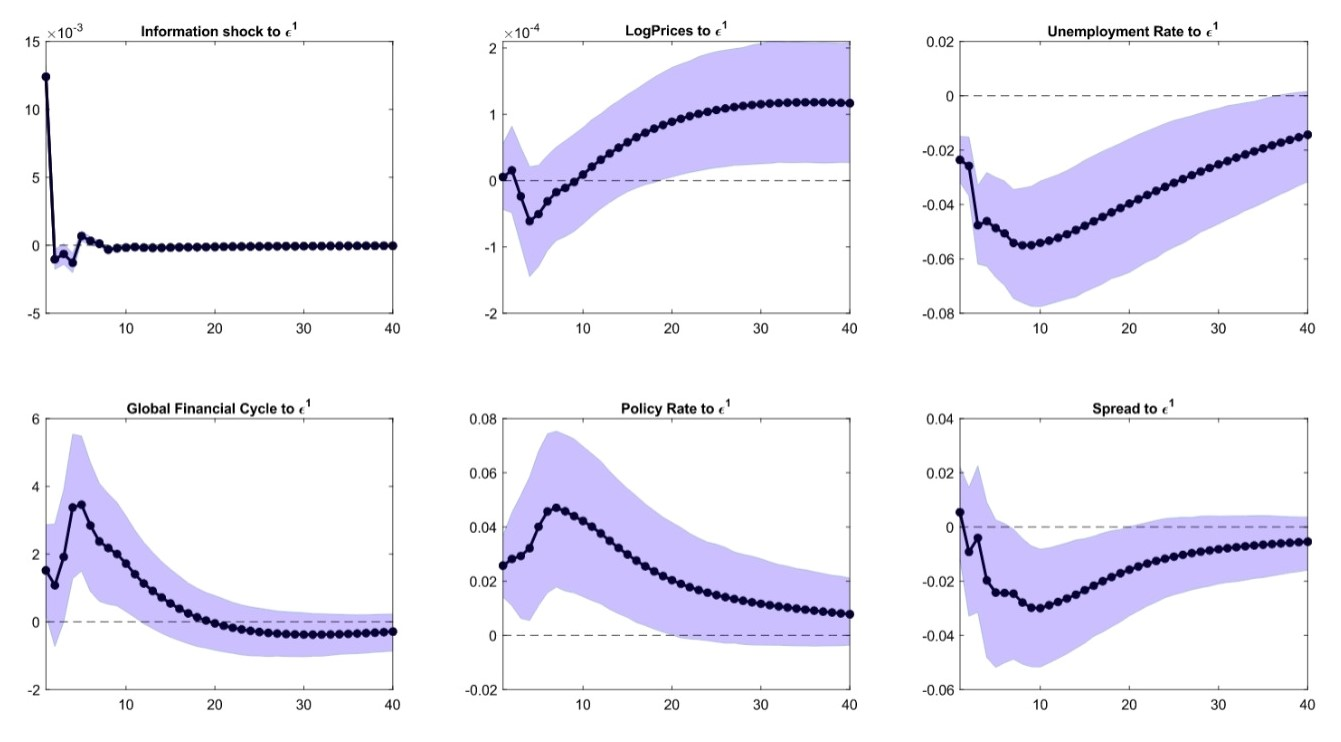
\includegraphics[scale=.5]{Graphs/IRF68.jpeg}
        \caption{IRFs for an information shock - 68\% confidence bands}
        \label{fig:IRF68}
    \end{figure}
% - - - - - - - - - - - - - - - - - - - - - - -

 % - - - - - - - - - FIGURE 2 - - - - - - - - -
    \begin{figure}[hp]
        \centering

        \begin{subfigure}{\textwidth}
            \centering
            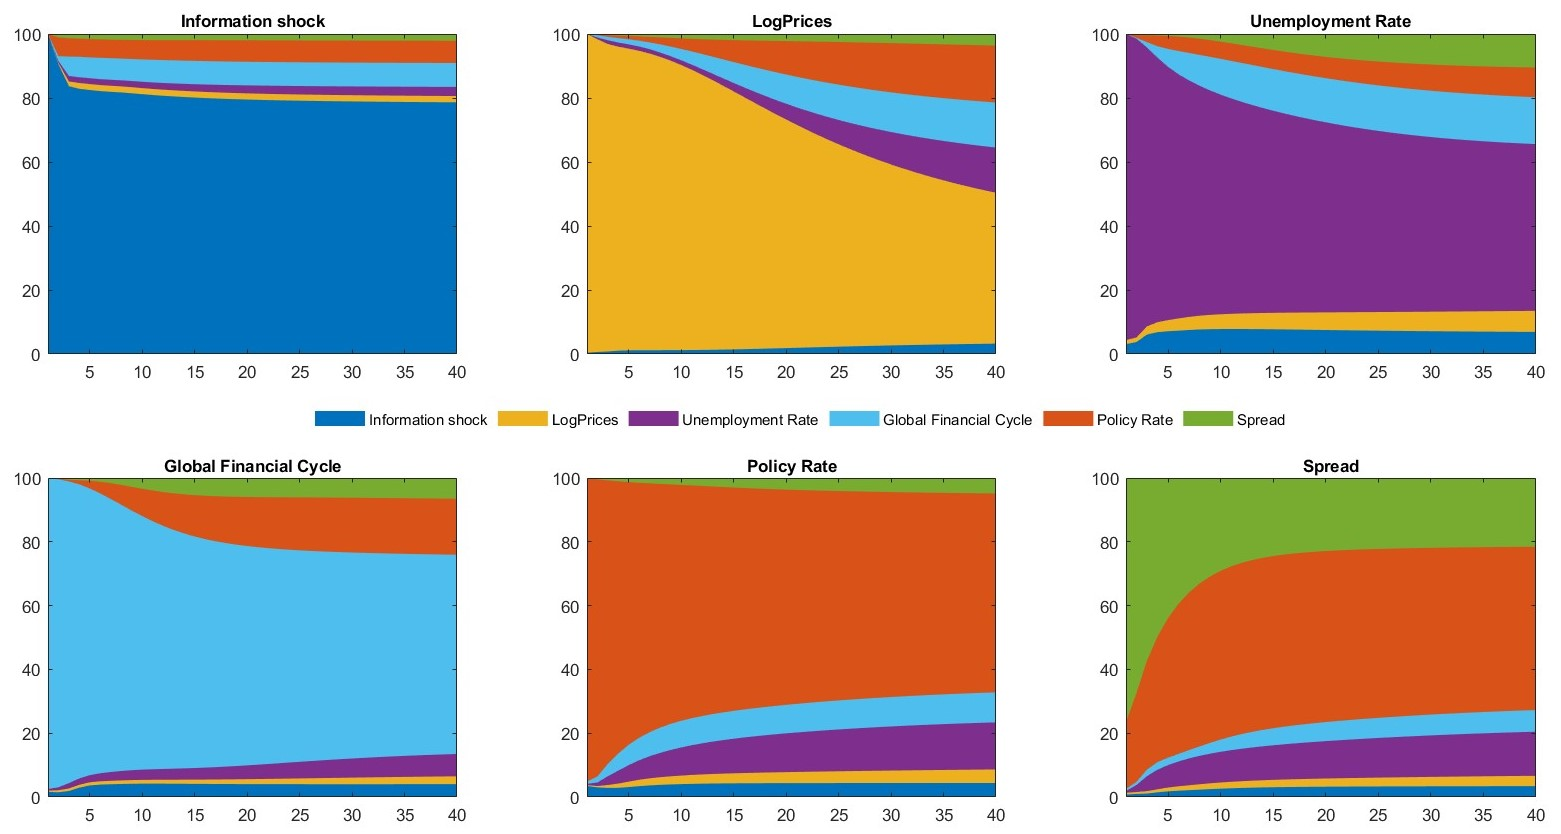
\includegraphics[scale=.32]{Graphs/forecast_err_variance_decomp.jpg}
            \captionsetup{font=scriptsize}
            \caption{Forecast Error Variance Decomposition}
            \label{fig:fevd}
        \end{subfigure}
        
        \vspace{0.2cm} % Adjust the vertical space between the rows
        
        \begin{subfigure}{\textwidth}
            \centering
            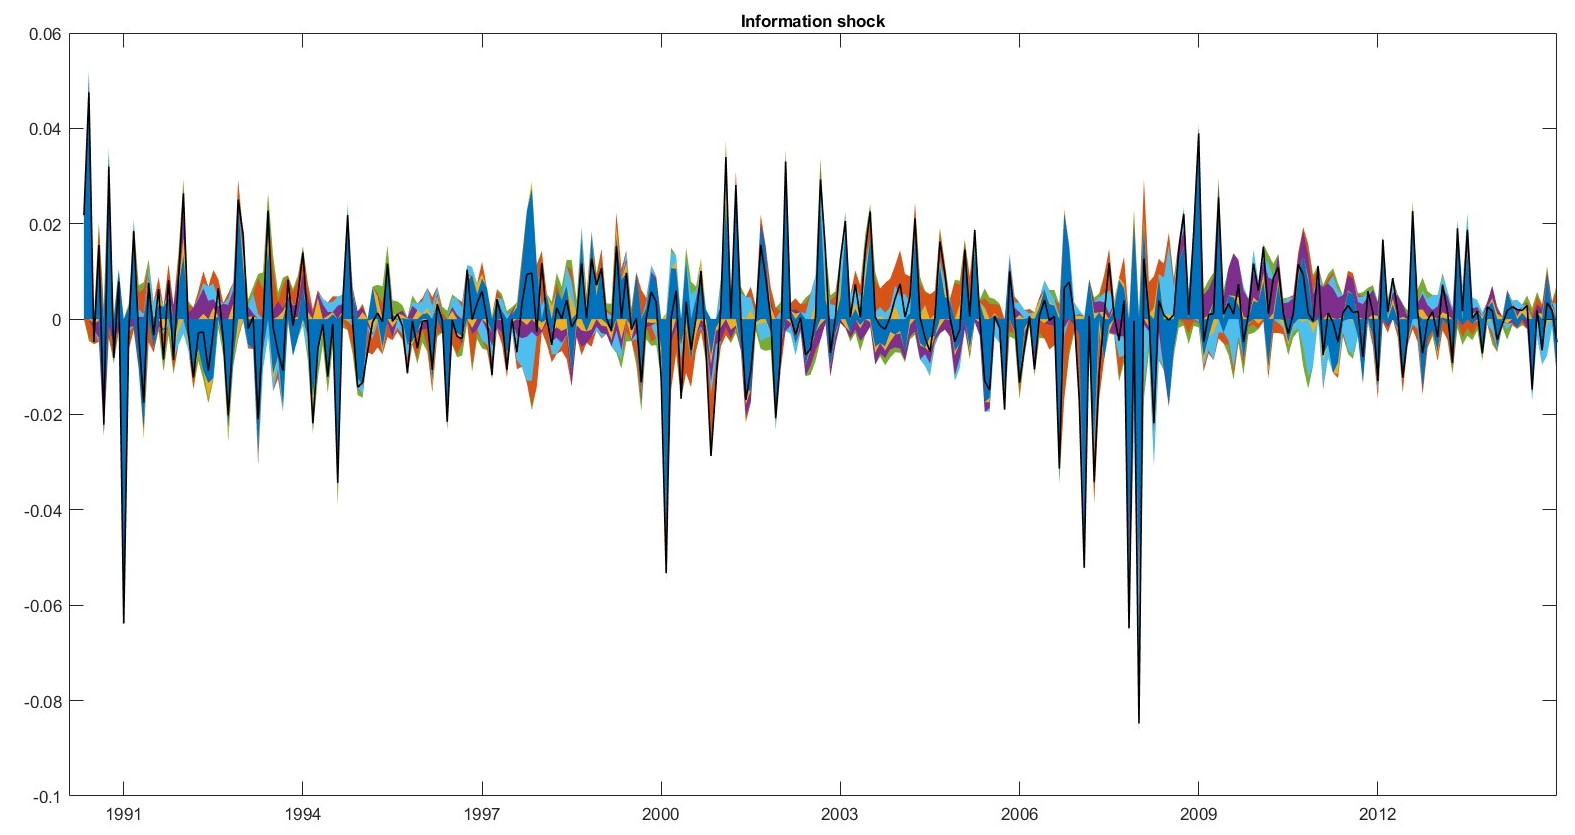
\includegraphics[scale=.32]{Graphs/INFO_FF4_HD.jpg}
            \includegraphics*[scale=0.22]{Graphs/Inkedlegend.jpg}
            \captionsetup{font=scriptsize}
            \caption{Information Shock Historical Decomposition}
            \label{fig:INFOhd}
        \end{subfigure}

        \vspace{0.2cm} % Adjust the vertical space between the rows
        
        \begin{subfigure}{\textwidth}
            \centering
            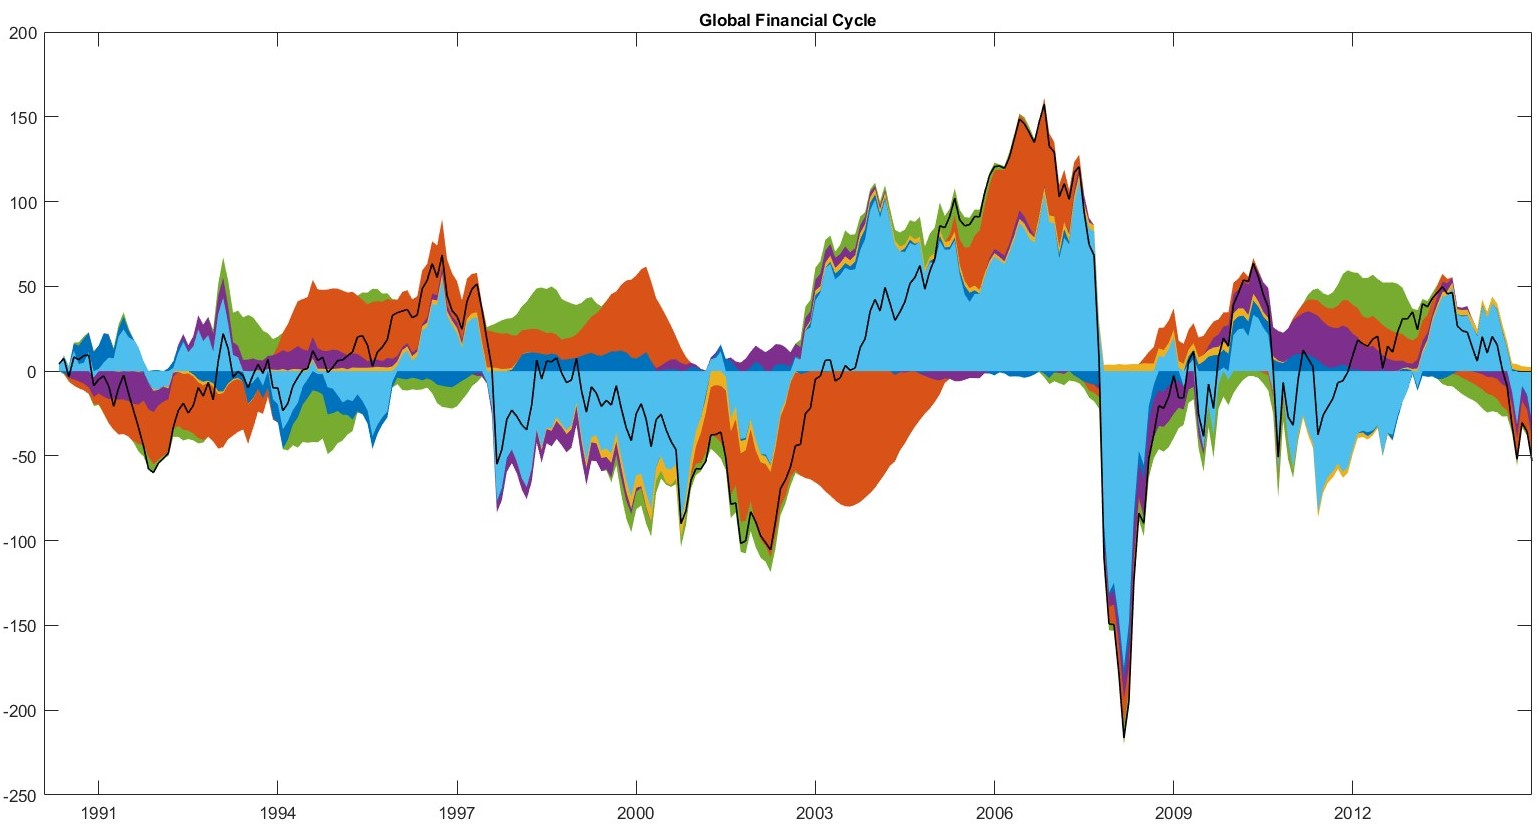
\includegraphics[scale=.32]{Graphs/GFC_HD.jpg}
            \includegraphics*[scale=0.22]{Graphs/Inkedlegend.jpg}
            \captionsetup{font=scriptsize}
            \caption{GFC Historical Decomposition}
            \label{fig:GFChd}
        \end{subfigure}

        \caption{ }
        \label{fig:additional_elements}
    \end{figure}
% - - - - - - - - - - - - - - - - - - - - - - -




\section{Discussion}

% > DISCUSSION OF IRFS (tutte VELOCEMENTE)
% > DISCUSSIONE DELLA IRF DEL GFC (NEL DETTAGLIO)
    % > MECCANISMI POSSIBILI
    % > CONFRONTO CON LA IRF A MP SHOCK

Comparing IRFs between the MP shock and the information shock gives insight into the formation of price puzzles seen in alternative specifications. 
On impact, both shocks cause an increase in the policy rate. However, Miranda-Agrippino and Ricco (2021) found a MP shock to be unequivocally contractionary, as opposed to what we can ascertain from the IRFs of Figure 1. 
An information shock signals that the CB expects a strong economy in the near future. In this case, an increase in the policy rate is followed by economic expansion. Prices rise, spreads fall and the GFC is stronger. 
This would only happen if the view that economic agents react to the information implicitly conveyed by the CB is correct, and my results point to this being the case.
    
An instrument such as Miranda-Agrippino and Rey's (2020), based on high-frequency surprises, does not properly disentangle the MP surprise from the information one may gives rise to price puzzles and other unexpected scenarios. This could potentially result in price puzzles and other unforeseen situations due to the conflated effects of these two factors. When separated, the MP shock is always followed by a contractionary response, and the information shock is followed by an expansionary response.
    %% source MARICCO 2021:
        %> Monetary policy surprises that contain both monetary policy shocks and demand shocks would blend the two effects reported in the figure and hence produce puzzles.
    

Figure 2 shows the Forecast Error Variance Decomposition (FEVD) for the information shock in panel (a), the information shock's historical decomposition in panel (b), and the GFC's historical decomposition in panel (c).

%vrs response to policy rate and to info shock 
FEVD is useful to understand how much a given variable contributes to the other variables. In panel (a), we can see that the policy rate has a hefty effect on the 10-year-3-month spread variable from the get go. Instead, the information shock mostly affects the unemployment rate, consistent with market agents adjusting labor demand depending on their expectations about economic fundamentals.
% GFC response to POLICY RATE and to INFO SHOCK
The GFC is mostly affected by the policy rate and the unemployment rate. 
However, given that the information shock originates from the US and provides insights into the state of the US economy, it is crucial to acknowledge that a non-negligible portion of the GFC is influenced by this particular shock. The impact of the information shock on the GFC cannot be dismissed or underestimated, as it plays a substantial role in shaping its dynamics.

% comment HD of the info shock and of the GFC (nei periodi di crisi l'info shock è più o meno capace di spiegare le fluttuazioni di GFC?)

    % INFO SHOCK:
        % > very noisy but with spikes around high uncertainty periods (1991 recession?, dotcom bubble in 2000, 2008 crisis)
The historical decomposition (HD) of the information shock in panel (b) is informative regarding the level of uncertainty surrounding economic conditions. 
The panel is noisy and does not suggest a systematic upward or downward contribution of the other variables to the shock's variability. 
Nevertheless, it is informative regarding the level of uncertainty surrounding economic conditions. 
It reveals that information shocks tend to exhibit greater variability and intensity during periods of significant economic stress, as seen in notable events such as the recessions around 1991, the dot-com bubble of the early 2000s, and the global financial crisis of 2008. These periods of high economic stress serve as crucial markers in the historical decomposition graph, underscoring the pronounced impact of information shocks during times of instability.
Interestingly, the unemployment component emerges as a more notable contributor to the observed variability following the onset of the 2008 crisis compared to the other events mentioned. % possible explanation



    % GFC:
        % > big nosedive in 2008 (expected)
        % > very affected by policy rate (see policy of the FED in the 2000s, might explain, and some history of the dot com bubble)
        % > policy rate was pushing up the GFC around 2006 -> too lenient FED was letting market overheat?
Relative to panel (b), panel (c) exhibits significantly reduced noise. 
The fluctuations observed in the GFC's HD reveal the US policy rate as a strong contributor, aligning with previously analyzed dynamics of the GFC and the role of the dollar in the international financial arena. 
However, although MP takes the lead in terms of spillover effects affecting the GFC, the role of information shocks remains non-negligible.
% DO NOT say it is countercyclical because HD gives the variance decomp for a specific var
The information shock also figures as a relevant component of the variation in GFC, usually in an attenuating manner. % CHECK CON DARIO, intendo che se GFC è negativo allora info shock tende ad essere positivo 


% - - - - - - CONCLUDING PARAGRAPH - - - - - - - %






\section*{References}
\begin{itemize}
    \item Cesa-Bianchi, Ambrogio. \url{https://github.com/ambropo/VAR-Toolbox}, VAR Toolbox for MatLab
    \item Christiano, Lawrence J., Martin Eichenbaum, and Charles L. Evans. \enquote{Nominal rigidities and the dynamic effects of a shock to monetary policy.} Journal of political Economy 113.1 (2005): 1-45.
    \item Miranda-Agrippino, Silvia, and Giovanni Ricco. \enquote{The transmission of monetary policy shocks.} American Economic Journal: Macroeconomics 13.3 (2021): 74-107.
    \item Miranda-Agrippino, Silvia, and Hélene Rey. \enquote{US monetary policy and the global financial cycle.} The Review of Economic Studies 87.6 (2020): 2754-2776.
    
\end{itemize}

\end{document}